\documentclass[12pt]{report}
\usepackage[utf8]{inputenc}
\usepackage[portuguese]{babel}

\usepackage{graphicx}
\usepackage{tabularx}
\usepackage[section]{placeins}
\usepackage{hyperref}
\usepackage{xspace}

\pagenumbering{arabic}

\begin{document}

\newcommand{\sajas}{\texttt{SAJaS}\xspace}
\newcommand{\jade}{\texttt{JADE}\xspace}
\newcommand{\repast}{\texttt{Repast 3}\xspace}
\newcommand{\massim}{\texttt{MASSim2Dev}\xspace}
\newcommand{\java}{\texttt{JAVA}\xspace}
\newcommand{\acl}{\texttt{ACL}\xspace}
\newcommand{\fipa}{\texttt{FIPA}\xspace}
\newcommand{\spotter}{\emph{spotter}\xspace}
\newcommand{\Spotter}{\emph{Spotter}\xspace}
\newcommand{\spotters}{\emph{spotters}\xspace}
\newcommand{\Producer}{\emph{Producer}\xspace}
\newcommand{\producer}{\emph{producer}\xspace}
\newcommand{\producers}{\emph{producers}\xspace}
\newcommand{\Transporter}{\emph{Transporter}\xspace}
\newcommand{\transporter}{\emph{transporter}\xspace}
\newcommand{\transporters}{\emph{transporters}\xspace}


  \begin{titlepage}
    \begin{center}
        \vspace*{1cm}
        
        \Huge
        \textbf{T05: Exploração de Marte}
        \vspace{0.5cm} \ \\
        \LARGE
        Agentes e Inteligência Artificial Distribuída
        
        \vfill
        
	
\includegraphics[width=0.6\textwidth]{FEUP_Logo}
	\break
        \small
        Novembro 2016
        
        \vfill
        
	\vspace{1.5cm}
        \normalsize{
	  Marina Camilo - up201307722 - up201307722@fe.up.pt \\
	  Diogo Ferreira - up201502853 - diogoff@fe.up.pt \\
	  Ângela Cardoso - up200204375 - angela.cardoso@fe.up.pt
        }
        
    \end{center}
  \end{titlepage}

\newpage
\tableofcontents

\clearpage
\chapter{Enunciado}

\section{Descrição do cenário}
No âmbito da unidade curricular de Agentes e Inteligência Artificial Distribuída, o nosso grupo propôs-se a implementar um Sistema Multi-Agente para simulação de um cenário de extração de minérios em Marte. Para tal, é necessário descobrir os minérios, extraí-los e transportá-los para a base. Sendo assim, no nosso sistema existem três tipos de Agentes:

\begin{itemize}
  \item \Spotter – Procura fontes de minérios e inspeciona-as para determinar se podem ser explorados. 
  \item \Producer – É chamado a uma fonte de minério por um \spotter para extrair o máximo de minério possível nessa fonte. 
  \item \Transporter – É alocado pelo \producer para carregar o minério obtido para a base.
\end{itemize}

De forma a facilitar a procura, todos os agentes podem localizar fontes de minérios e enviar a sua localização para os \spotters que os analisarão. A escolha do \producer por parte do \spotter segue um protocolo de negociação. A alocação dos \transporters a uma determinada fonte segue também um protocolo de negociação, iniciado pelo \producer. Esta alocação, terá em conta a quantidade de minério a transportar, de modo a determinar mais corretamente o número necessário de \transporters.

\section{Objetivos do trabalho}

Um dos objetivos deste trabalho é implementar os agentes de forma a que a simulação da exploração seja tão eficiente quanto possível. Para tal serão estudadas várias alternativas de implementação, de forma a determinar qual a melhor abordagem. No caso dos agentes do tipo \spotter, tencionamos usar algoritmos de distribuição do espaço a explorar entre eles, para que cubram toda a região mais rapidamente. Em relação aos \producers e \transporters, pretendemos instalar protocolos de negociação que garantam que o melhor agente é escolhido para a tarefa.

O nosso maior objetivo é utilizar este projeto como forma de melhor interiorizar os conceitos dos Sistemas Multi-Agente, nomeadamente ganhando uma maior familiaridade com as plataformas que permitem implementar e simular estes sistemas.

\section{Resultados esperados e forma de avaliação}

Para podermos ver resultados mais rapidamente, inicialmente serão implementadas apenas as funcionalidades mais básicas de cada tipo de agente. Como tal, a primeira fase de avaliação preocupar-se-á essencialmente em garantir que cada agente faz aquilo que é suposto.

Numa segunda fase, introduziremos as restrições pretendidas para a simulação, nomeadamente a capacidade limitada dos \transporters e o facto de todos os agentes poderem detetar minério nas suas deambulações. Uma vez realizadas estas alterações aos agentes básicos, a avaliação geral levará em conta o tempo que a simulação demora a correr e o número de passos efetuados por todos os agentes. Usando estas métricas, dados vários tamanhos para o espaço inicial a explorar, iremos determinar a complexidade do nosso sistema. Para podermos melhorar cada componente individual, calcularemos também métricas mais finas, como o tempo de espera médio e máximo, quando é invocado um \producer ou um \transporter, ou o tempo de exploração do terreno pelos \spotters consoante o seu número.

Com as métricas obtidas após a segunda fase de implementação, analisaremos diferentes algoritmos de forma a tornar mais eficiente esta demanda. Nomeadamente, avaliaremos qual a alocação mais eficiente de agentes, se o mapa fica corretamente dividido entre os \spotters e se o tempo de simulação foi o mínimo para o caso em questão.


\chapter{Plataforma/Ferramenta}

\section{Para que serve}

  \subsection{\jade}
  O \jade, \emph{Java Agent DEvelopment Framework}, é um software que permite desenvolver sistemas baseados em agentes. Os agentes são distribuídos por \emph{containers} que podem estar em máquinas diferentes, cada um utiliza uma \emph{thread}. 

  \subsection{\repast}
  O \repast, \emph{Recursive Porous Agent Simulation Toolkit}, é uma ferramenta de simulação baseada em agentes, que permite construir simulações locais à máquina com diversos agentes. O processamento de cada agente é distribuído por \emph{threads}.

  \subsection{\sajas}
  O \sajas, \emph{Simple API for JADE-based Simulations}, é uma ferramenta que se propõe servir de ponte entre o desenvolvimento e a simulação de Sistemas Multi-Agente. Desta forma, através do \sajas, podemos tomar vantagem dos benefícios do \jade e do \repast.

\section{Descrição das características principais}

  \subsection{\jade}
  O \jade é uma ferramenta totalmente escrita em \java, que suporta troca de mensagens \acl, seguindo a especificação \fipa. Além disso, possui um sistema de gestão de agentes e um sistema de páginas amarelas. Como os agentes estão distribuídos por contentores que podem estar em máquinas diferentes, permite ter agentes remotos. Os agentes podem migrar entre contentores e ser clonados. Esta plataforma possui ainda uma série de ferramentas que simplificam a administração e o desenvolvimento de aplicações, tais como:
  \begin{itemize}
   \item agente de monitorização remota - interface gráfico para monitorizar a atividade dos agentes;
   \item agente pateta - permite trocar mensagens com outros agentes;
   \item agente inspetor - permite inspecionar outros agentes;
   \item agente introspetivo - permite monitorizar o ciclo de vida de um agente.
  \end{itemize}
  A implementação de agentes em \jade é feita recorrendo a comportamentos, que determinam as tarefas a executar pelos agentes consoante o contexto. 
  
  \subsection{\repast}
  O \repast suporta simulação de espaços físicos, representação 2D e 3D e análise em tempo real. Possui uma barra de ferramentas para controlar as simulações, um interface gráfico para manipular os parâmetros. Permite recolher dados em vários formatos, incluindo vários tipos de gráficos. A interação entre os agentes pode ser visualizada graficamente. Os espaços físicos simulados podem ser de variados tipos, como por exemplo, grelhas hexagonais ou retangulares, espaços contínuos ou redes. Além de poderem ser corridas com recurso ao interface gráfico, as simulações podem também ser lançadas em \emph{batch}.
  
  O simulador discreto considera unidades de tempo - \emph{ticks} ou passos. Os eventos são planeados para ocorrer em \emph{ticks} específicos e assim é respeitada a ordem dos acontecimentos. Uma simulação considera um conjunto de agentes, cujos comportamentos são controlados recorrendo ao plano.

  \subsection{\sajas}
  O \sajas permite construir um Sistema Multi-Agente tal como é feito em \jade, existindo até uma ferramenta (\massim) que traduz código \jade para \sajas (e vice-versa), alterando as classes importadas. Ao contrário do \jade, permite ainda, recorrendo para isso ao \repast, a simulação deste tipo de sistemas. Além disso, o \sajas permite ainda obter melhores performances do que numa simulação construída em \jade, que teria que considerar algum tipo de agente representado o `mundo'.

\section{Realce das funcionalidades relevantes para o trabalho}

Com o suporte do \jade são feitos os protocolos de comunicação entre os diferentes agentes, utilizando mensagens \acl. Usando o \repast torna-se
fácil simular um espaço físico, popular o espaço com os agentes construídos em \jade, desenhá-los e finalmente vê-los em ação, obtendo gráficos relativos à sua performance. O \sajas permite-nos recorrer a estas duas ferramentas simultaneamente, construindo e simulando o nosso sistema de forma eficiente.

\chapter{Especificação}

\section{Identificação e caracterização dos agentes (arquitetura, comportamento, estratégias)}

Tal como descrito acima, o nosso sistema tem três tipos de agentes. De seguida descrevem-se mais detalhadamente estes agentes e a forma como decidimos implementá-los.

\subsection{\Spotter}
A nossa intenção é que cada \spotter tenha a sua região conexa do espaço para explorar. Uma vez definida essa região, a estratégia do \Spotter é simples, inspeciona cada célula consecutivamente, determinando se contém minério extraível e guardando registo desta informação. Sempre que encontra minério extraível, entra em contacto com todos os \producers para negociar e decidir qual deles será chamado para extrair o minério.

Numa segunda fase, depois de introduzirmos as restrições no sistema, os \spotters receberão notificações dos restantes agentes quando estes últimos detetarem minérios. O \spotter a quem estiver atribuída essa célula ficará com a responsabilidade de a inspecionar e determinar se o minério pode ser explorado. Em princípio, o mesmo acontecerá na primeira movimentação dos \spotters para as suas regiões. Isto é, eles detetaram minério e espalharão essa informação, mas apenas inspecionam a sua região.

Mais tarde, pretendemos explorar diferentes formas de dividir o espaço entre os \spotters, para determinar qual a melhor forma. Entre outras coisas, para que os \producers iniciam a sua atividade mais cedo, pode ser melhor que na movimentação inicial para as suas regiões os \spotters inspecionem minério encontrado, mesmo que não esteja nas suas regiões.

\subsection{\Producer}
Os \producers entram em ação assim que é encontrado minério extraível por um \spotter. Nesse momento cada um deles terá que determinar o esforço necessário para se deslocar ao local e extrair o minério. Esse esforço corresponde à distância (em passos) a que o \producer se encontra do local, mais o tempo (em passos) que ele demorará a terminar a sua tarefa atual, caso esteja a extrair minério, mais o tempo que demorarão todas as outras tarefas com as quais já se tenha comprometido. Para esse efeito, cada \producer deve guardar uma fila contendo informação sobre as suas extrações, em particular o tempo que cada uma delas demora, incluindo a deslocação da sua posição anterior até ao local da extração.

Numa primeira fase de implementação, assumiremos princípios muito simples relativamente à extração, nomeadamente que requer sempre o mesmo número de passos. Mais tarde, a quantidade e/ou profundidade do minério poderão ser levadas em conta para determinar o tempo de extração.

\subsection{\Transporter}
Os \transporters iniciam a sua atividade quando são contactados para transportar minério. À semelhança do que acontece com os \producers, nesse momento terão de calcular o esforço que necessitam para se deslocarem ao local. Inicialmente, dado que se assume capacidade ilimitada e transporte do minério para a base imediatamente, o esforço corresponde apenas à soma das distâncias que o \transporter terá que percorrer para se deslocar entre os locais para os quais foi convocado e a base. 

Quando for considerada a limitação de carga, o \transporter poderá ter vários comportamentos diferentes que serão estudados quanto à sua eficiência. Ele poderá regressar à base apenas quando atinge a carga máxima, ou então regressar sempre que não estiver ocupado com transportes. Quando informar os \producers do esforço que necessita para chegar até um local terá que considerar quais as viagens à base que fará e também qual o espaço que terá disponível quando lá se deslocar. Tudo isso será considerado pelo \producer ao escolher o seu \transporter. Se o tempo permitir, consideraremos ainda a possibilidade de vários \transporters serem alocados à mesma tarefa, caso a quantidade de minério assim o exija ou essa pareça ser a ação mais eficiente.

\section{Protocolos de interação}

\subsection{Divisão de espaços}
Inicialmente cada \spotter deve acordar com os restantes a região do espaço que será sua para explorar. 

\begin{figure}[h]
  \centering
    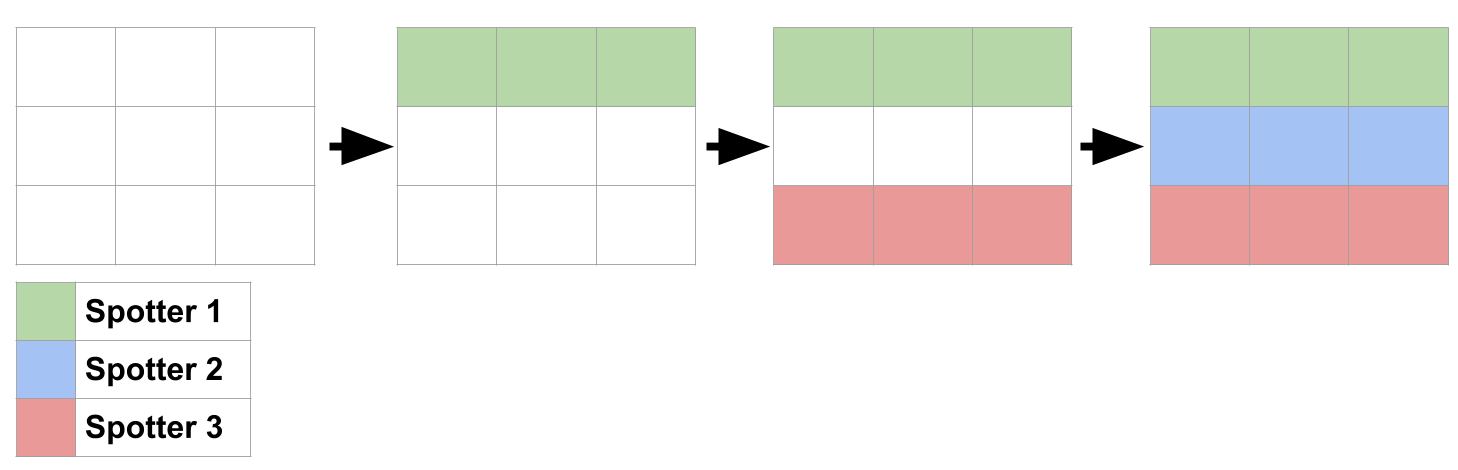
\includegraphics[width=0.6\textwidth]{spotter-spaces}
  \caption{\small{Alocação simples por linhas}}
  \label{spotter-spaces}
\end{figure}

Sendo o espaço uma matriz retangular, numa primeira fase de implementação, assumiremos que o número de \spotters é igual ao número de linhas da matriz, de forma a que cada \spotter fique com uma linha. A Figura~\ref{spotter-spaces} ilustra esta divisão para três \spotters.

\begin{figure}[h]
  \centering
    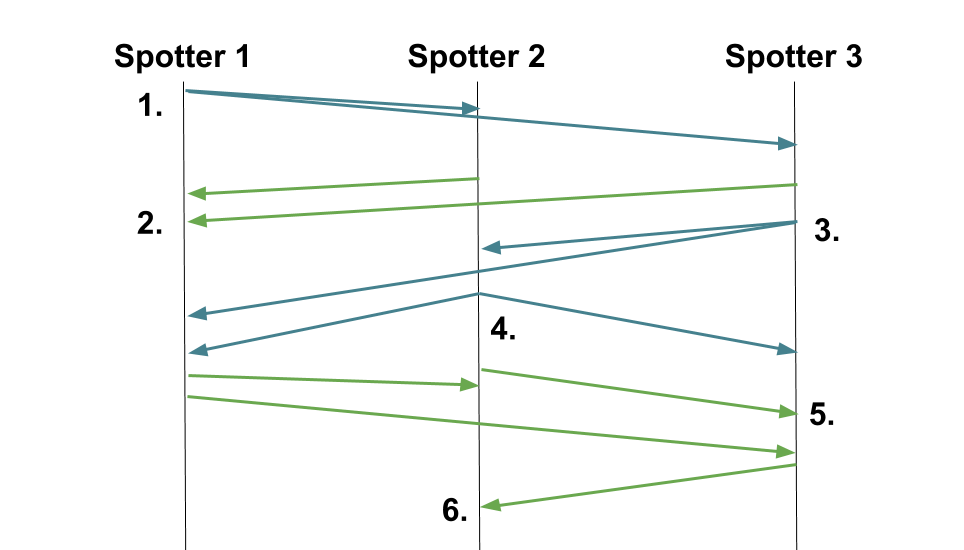
\includegraphics[width=0.6\textwidth]{spotter-agreement}
  \caption{\small{Diagrama temporal das comunicações entre \spotters}}
  \label{spotter-agreement}
\end{figure}  

Cada \spotter escolhe uma linha e depois comunica aos restantes a sua escolha, que ficam encarregues de confirmar a afetação. Esta comunicação, correspondente ao exemplo acima, é ilustrada na Figura~\ref{spotter-agreement}:
\begin{enumerate}
	\item \spotter 1 comunica aos restantes o espaço que pretende explorar;
    \item \spotter 1 recebe confirmação dos restantes e fica afeto ao espaço que pretendia;
    \item \spotter 3 comunica aos restantes o espaço que pretende explorar;
    \item \spotter 2 comunica aos restantes o espaço que este pretende explorar;
    \item \spotter 3 recebe confirmação dos restantes e fica afeto ao espaço que pretendia;
    \item \spotter 2 recebe confirmação dos restantes e fica afeto ao espaço que pretendia.
\end{enumerate}

Neste exemplo, assumiu-se que não há sobreposição nas escolhas. Nessa caso, alguns dos \spotters terão que desistir das suas escolhas e comunicar novas, aguardando confirmação.

\FloatBarrier
\subsection{Afetação de \producers}
Uma vez encontrado minério é necessário chamar um \producer para o extrair. O \spotter envia então a posição do  minério a todos os \producers. 
Estes respondem com o valor do esforço de que necessitarão para se deslocar até ao local. 
O \spotter escolhe o \producer com o menor esforço e comunica com ele, pedindo para confirmar a afetação. 
Caso seja recusado, porque o \producer foi afeto a outro minério entretanto, o \spotter repete o processo desde o início.

\begin{figure}[h]
  \centering
    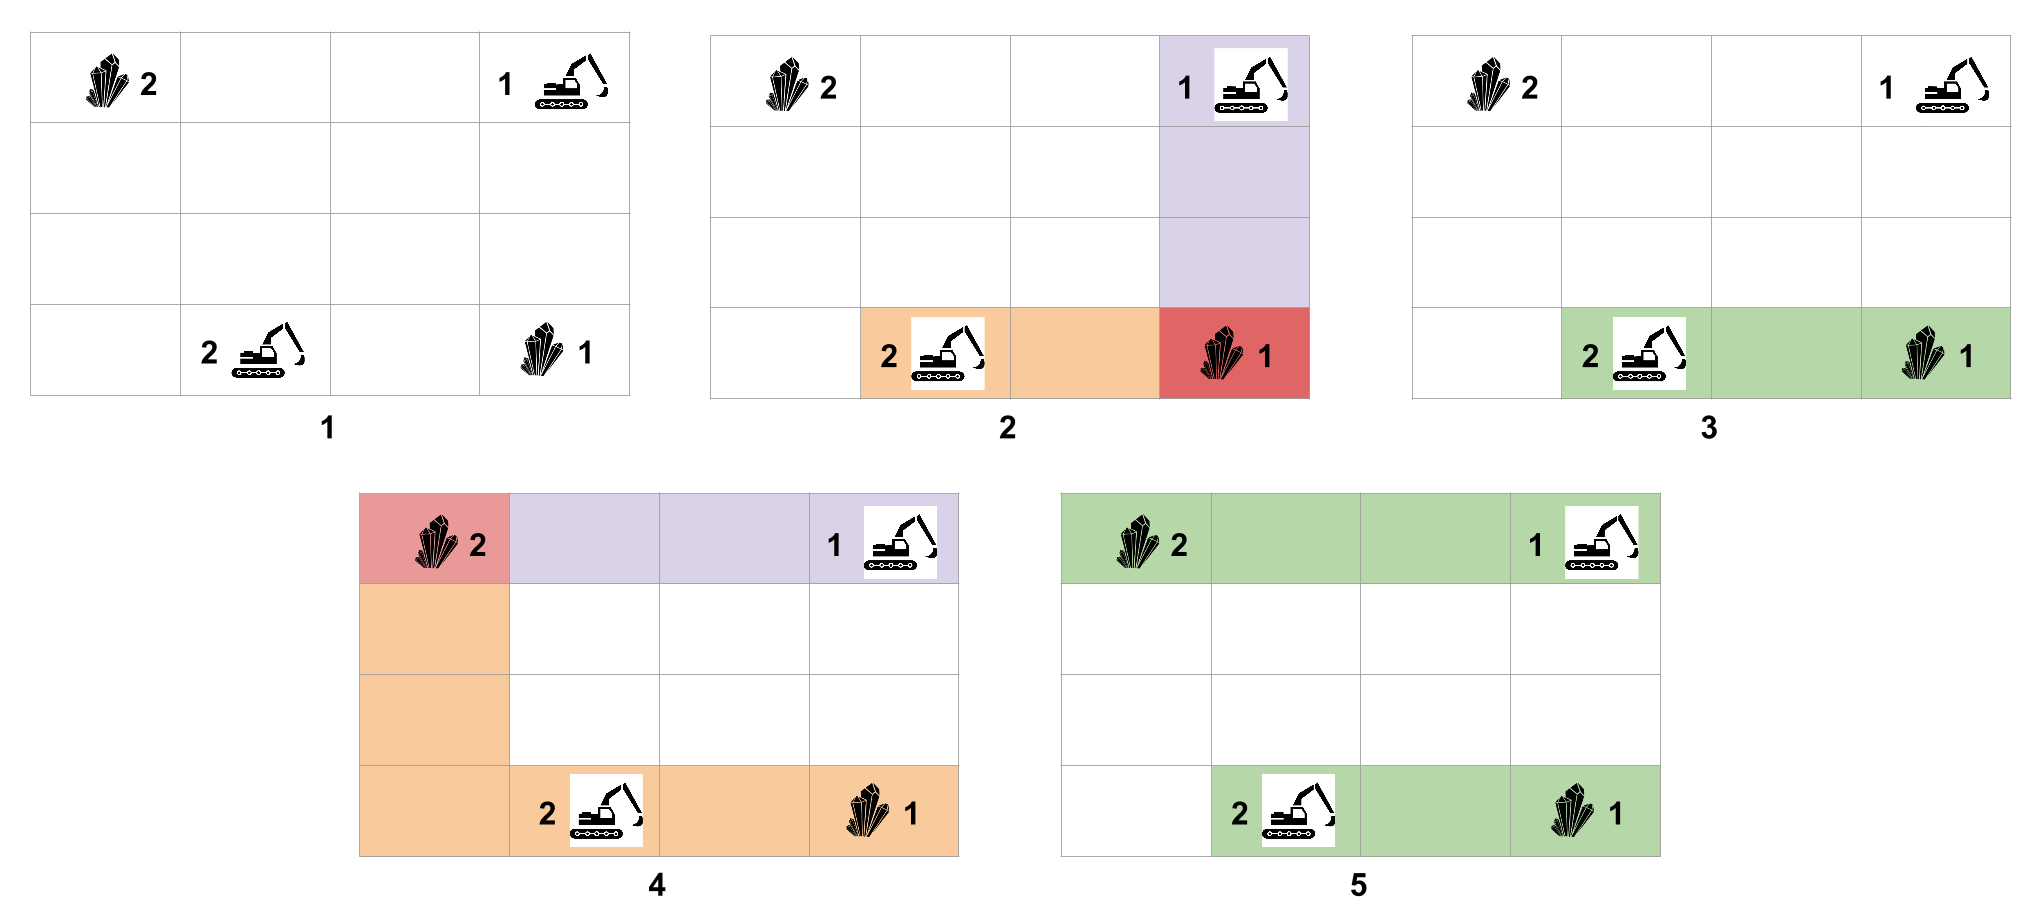
\includegraphics[width=0.8\textwidth]{producer-scheduling}
  \caption{Exemplo de afetação de \producers}
  \label{producer-scheduling}
\end{figure}

A Figura~\ref{producer-scheduling} exemplifica o processo de escolha de \producers para os minérios encontrados pelos \spotters 1 e 2. 
Neste caso, ficou o \producer 2 afeto ao minério do \spotter 1 e o \producer 1 afeto ao minério do \spotter 2.

\FloatBarrier
\subsection{Afetação de \transporters}
Após a extração do minério é necessário transportá-lo para a nave-mãe. 
O \producer que acabou de extrair o minério tem que selecionar um \transporter, do mesmo modo que o \spotter seleciona um \producer. 
Cada \transporter comunica o valor do esforço e o minério que consegue transportar possibilitando o \producer de escalonar os diferentes agentes.

\begin{figure}[h]
  \centering
    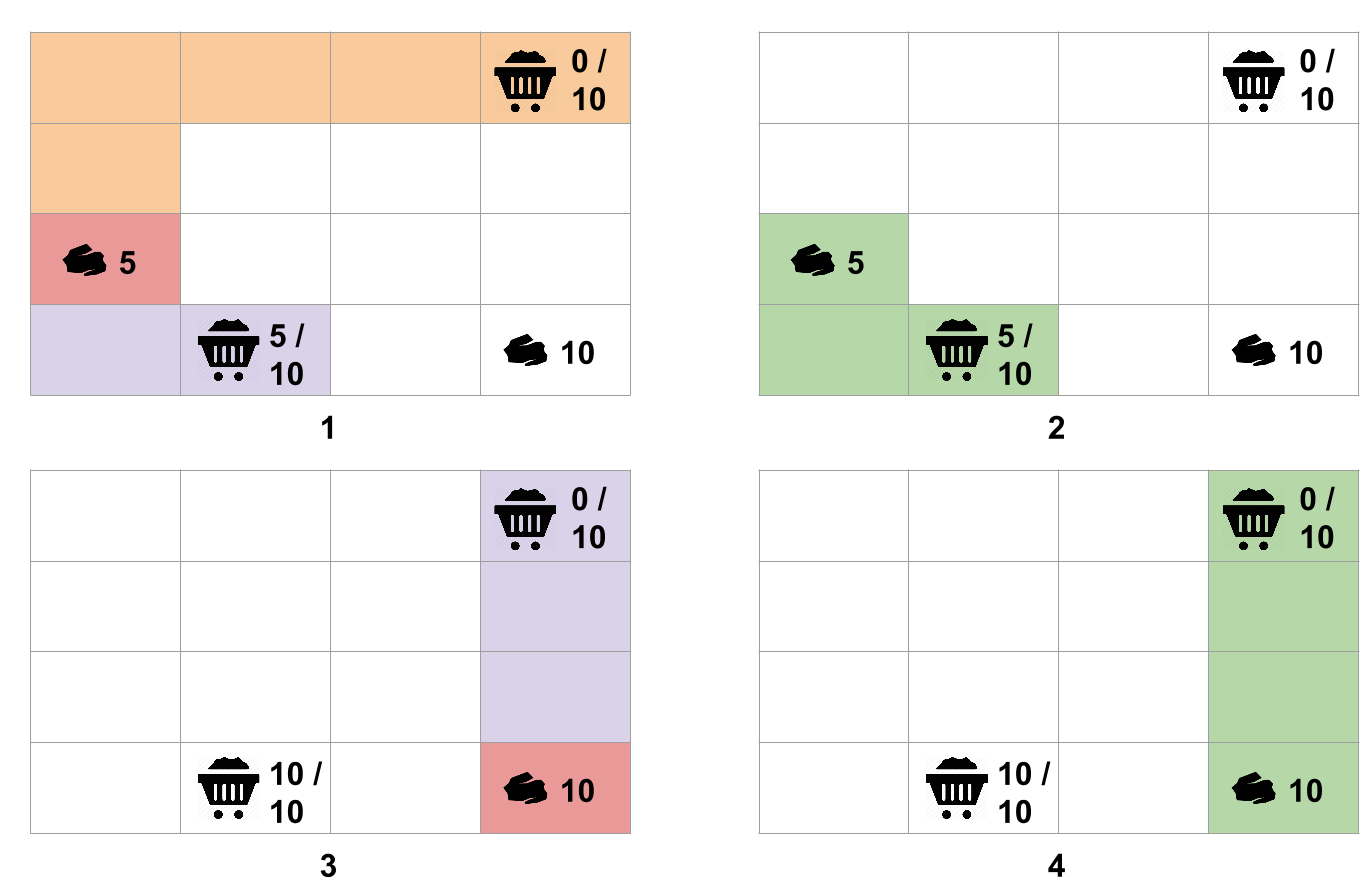
\includegraphics[width=0.8\textwidth]{transporter-scheduling}
  \caption{Exemplo de afetação de \transporters}
  \label{transporter-scheduling}
\end{figure}

A Figura~\ref{transporter-scheduling} exemplifica o processo de escolha de \transporters para os minérios extraídos por dois \producers. Consideramos ainda as quantidades de minério extraídas, a capacidade e carga corrente dos \transporters. Estas restrições irão influenciar a forma como se negoceia a afetação dos \transporters numa fase mais avançada da implementação.

\newpage
\section{Faseamento do projeto}

A forma como decidimos implementar o nosso projeto tem como objetivo principal garantir que obtemos resultados e temos um protótipo funcional desde cedo. Sendo assim, o nosso plano é:
\begin{enumerate}
	\item construir ambiente de simulação em \repast;
	\item implementar agente do tipo \spotter apenas com as tarefas de dividir o território, explorar e mapear os seus achados;
    \item implementar agente do tipo \producer, com a função de se descolar aos locais e extrair o minério; 
	\item estabelecer a comunicação entre \spotters e \producers;
	\item implementar agente \transporter sem limite de capacidade e apenas com a função básica de transportar;
	\item estabelecer a comunicação entre \producers e \transporters;
	\item retirar a limitação do número de \spotters ser função do número de linhas da matriz;
	\item introduzir as restrições de capacidade e quantidade de minério nos \transporters e na sua negociação com os \producers;
	\item permitir que todos os agentes detetem minério nas suas deslocações e comuniquem com os \spotters;
	\item estudar formas diferentes de distribuição dos \spotters pelo espaço;
	\item estudar outras alternativas de afetação dos \producers e \transporters e determinar a mais eficiente.
\end{enumerate}

\chapter{Recursos}

\section{Bibliografia}
\section{Software}

\end{document}